\section{Sampling}
Later in ou study, we will use the trajectory of the Earth in the heliocentric renferential in order to evaluate our models. To be more precise, the score of a model will be the difference between the real Earth's trajectory and the trajectory we estimate with the values or functions we find.\\
In order to do that, we need to be able to sample the Earth path in that referential. Let us study the Earth in the heliocentric renferential.\\

\noindent
\textbf{System:} Earth, assimilated to a material point of mass \(M_{T}\)\\
\textbf{Referential:} Galilean assumed heliocentric renferential\\
\textbf{Coordinates System:} Polar coordinates\\
\textbf{Balance of forces:} Attraction force of the Sun of mass \(M_{S}$: $\vec{F} = -G\frac{M_{T} M_{S}}{r^{2}}\vec{e_{r}}\)\\

According to Newton's second law:
\[
\begin{align*}
M_{T}\vec(a) = \vec{F}
& \iff
\begin{equation}
    \begin{cases}
    M_{T}(\ddot{r}-r\dot{\theta}^{2}) = -G\frac{M_{T} M_{S}}{r^{2}}\\
    M_{T}(2\dot{r}\dot{\theta}+r\ddot{\theta}) = 0
    \end{cases}
\end{equation}
& \iff
\begin{equation}
    \begin{cases}
    \ddot{r} = r\dot{\theta}^{2}-G\frac{M_{T} M_{S}}{r^{2}}\\
    \ddot{\theta} = -\frac{2\dot{r}\dot{\theta}}{r}
    \end{cases}
\end{equation}
\end{align*}
\]

In order to sample the Earth's trajectory, we perform two Euler methods simultaneously: the first one allows us to obtain the speed and the second one gives us the actual position.
\[
\begin{equation}
    \begin{cases}
    r_{n+1} = r_{n} + \dot{r_{n}} \delta t\\
    \theta_{n+1} = \theta_{n} + \dot{\theta_{n}} \delta t
\end{cases}
\end{equation}

\begin{equation}
    \begin{cases}
    \dot{r_{n+1}} = \dot{r_{n}} + \ddot{r_{n}} \delta t\\
    \dot{\theta_{n+1}} = \dot{\theta_{n}} + \ddot{\theta_{n}} \delta t
    \end{cases}
\end{equation}

\text{with}
\delta t = \frac{365,25 \times 24 \times 3600}{1024}
\text{ as we want to sample 1024 points.}
\]

We also have to set the initial conditions. Let us suppose we start to sample when the Earth is located at the perihelion, as the distance between the Earth and the Sun and the speed of the Earth at this point are known, we obtain the following conditions:
\[
\begin{equation}
    \begin{cases}
    r_{0} = 147,1 \times 10^{9}\\
    \theta_{0} = \pi\\
    \dot{r_{0}} = 0\\
    \dot{\theta_{0}} = \frac{2\pi \times 30,2 \times 10^{3}}{\pi \left( 3 (a + b) - \sqrt{(3a + b) \times (a + 3b)}\right)}
    \end{cases}
\end{equation}

% \text{with}
% a = 1521,0 \times 10^{8}
% \text{ and }
% b = 1471,0 \times 10^{8}
% \text{ the distances between the Earth and the Sun respectively at the aphelion and at the perihelion.}
\]
with \(a = 1521,0 \times 10^{8}\) and \(b = 1471,0 \times 10^{8}\) the distances between the Earth and the Sun respectively at the aphelion and at the perihelion.

With this set of equations we can write a program that precisely compute 1024 positions of the Earth while orbiting around the Sun.

\begin{figure}[H]
    \center
    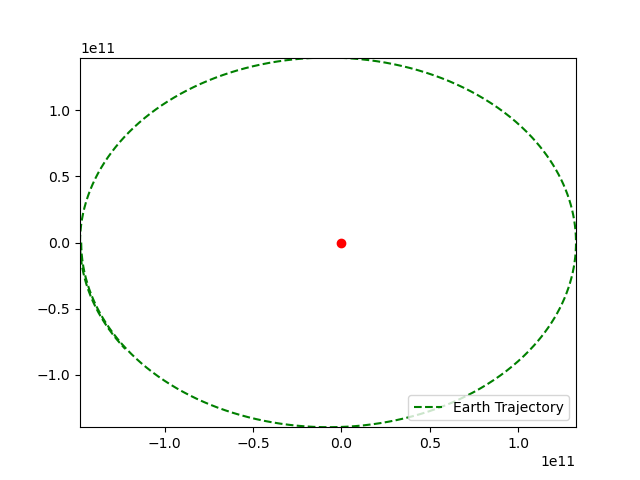
\includegraphics[scale=.5]{img/earth_trajectory_test.png}
    \caption{Earth trajectory around the Sun (1024 points sampling)}
\end{figure}